% !TeX root = ../Doc_especific_mse_anchovy.tex

\subsection{Error de proceso del reclutamiento}

El error de proceso en el modelo operativo utiliza la misma desviación estándar del modelo base y considera la autocorrelación de los reclutamientos históricos tomados de las estimaciones del modelo base de evaluación de stock. Las desviaciones de los reclutamientos para el período de la proyección son generadas de una distribución log-normal, con una desviación estándar y factor de autocorrelación al primer retraso reportadas por el modelo de evaluación (Figura 4). 
\newline

Para el modelo operativo base, la desviación estándar para las desviaciones de los logaritmos de los reclutamientos para la anchoveta fue de 0.82 con un factor de autocorrelación de -0.1868. En la Figura 5 se muestra un ejemplo de las desviaciones de los reclutamientos para nueves simulaciones.

\begin{figure}[H]
    \centering
    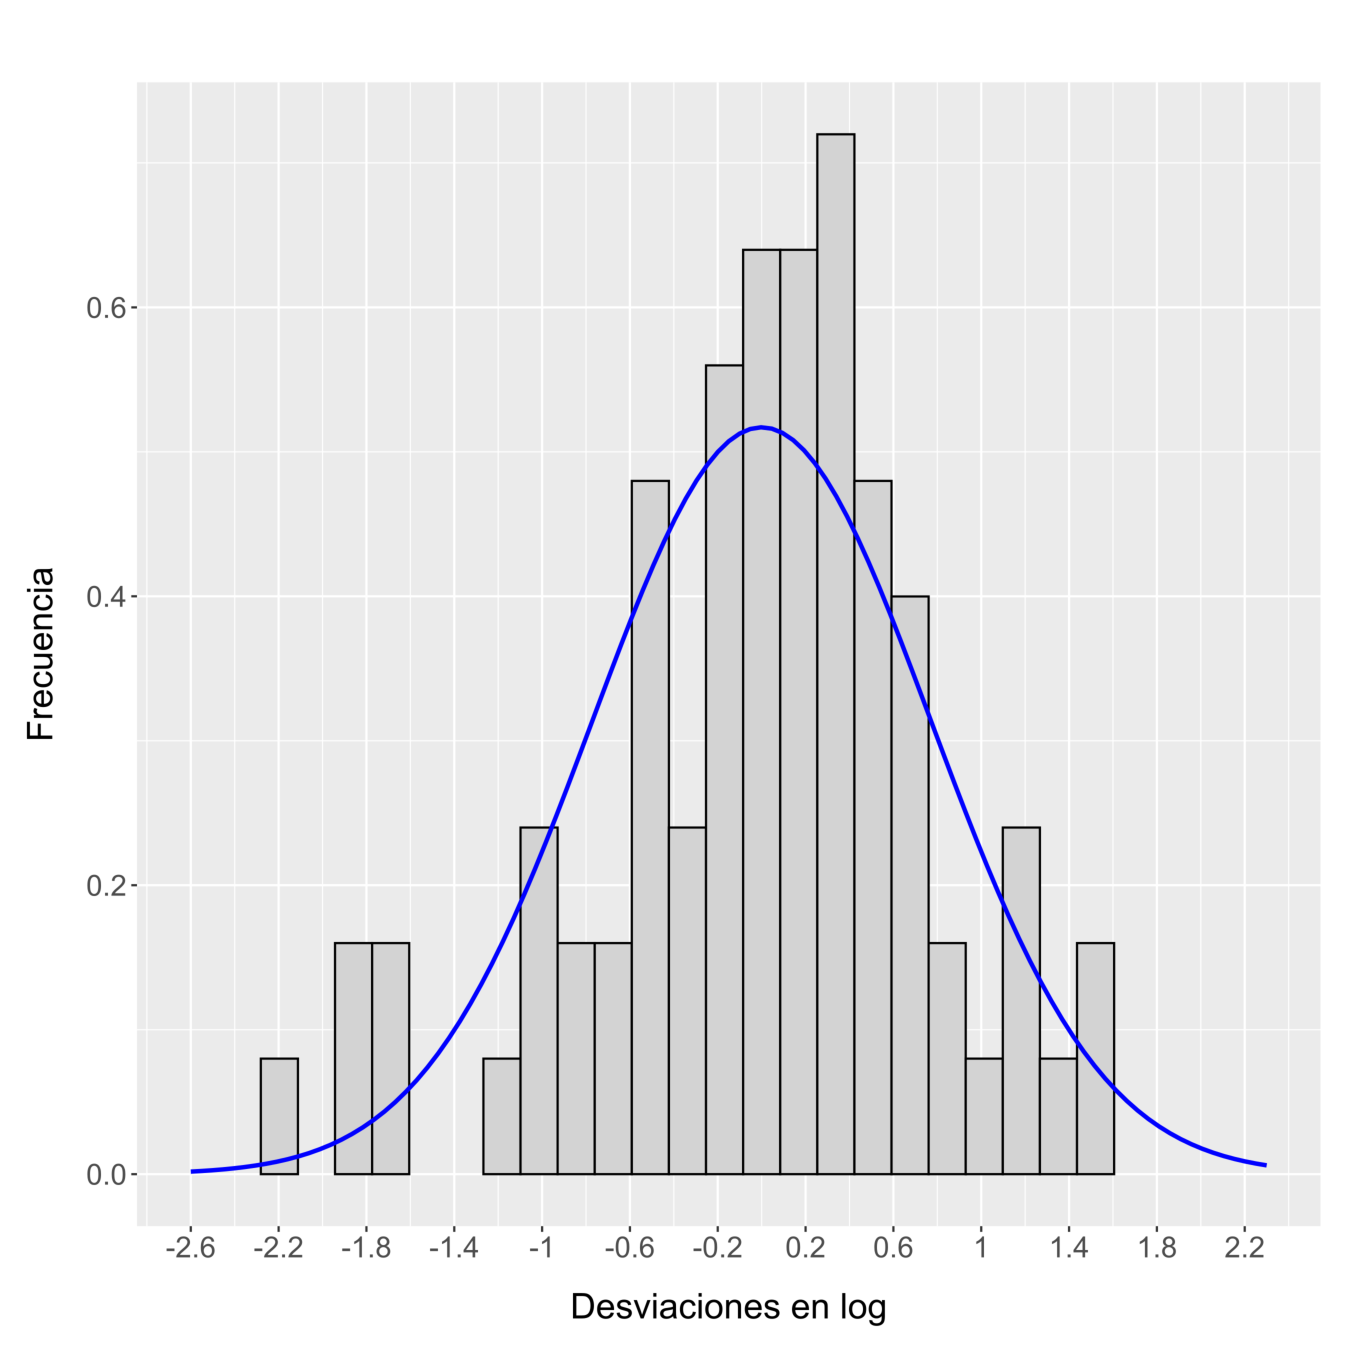
\includegraphics[scale=0.35]{figura4.pdf}
    \caption{Distribución de las desviaciones de los logarítmicos de los reclutamientos para el stock de anchoveta, la línea azul representa el ajuste de una distribución normal.}
    \label{fig:figura4}
\end{figure}

\begin{figure}[H]
    \centering
    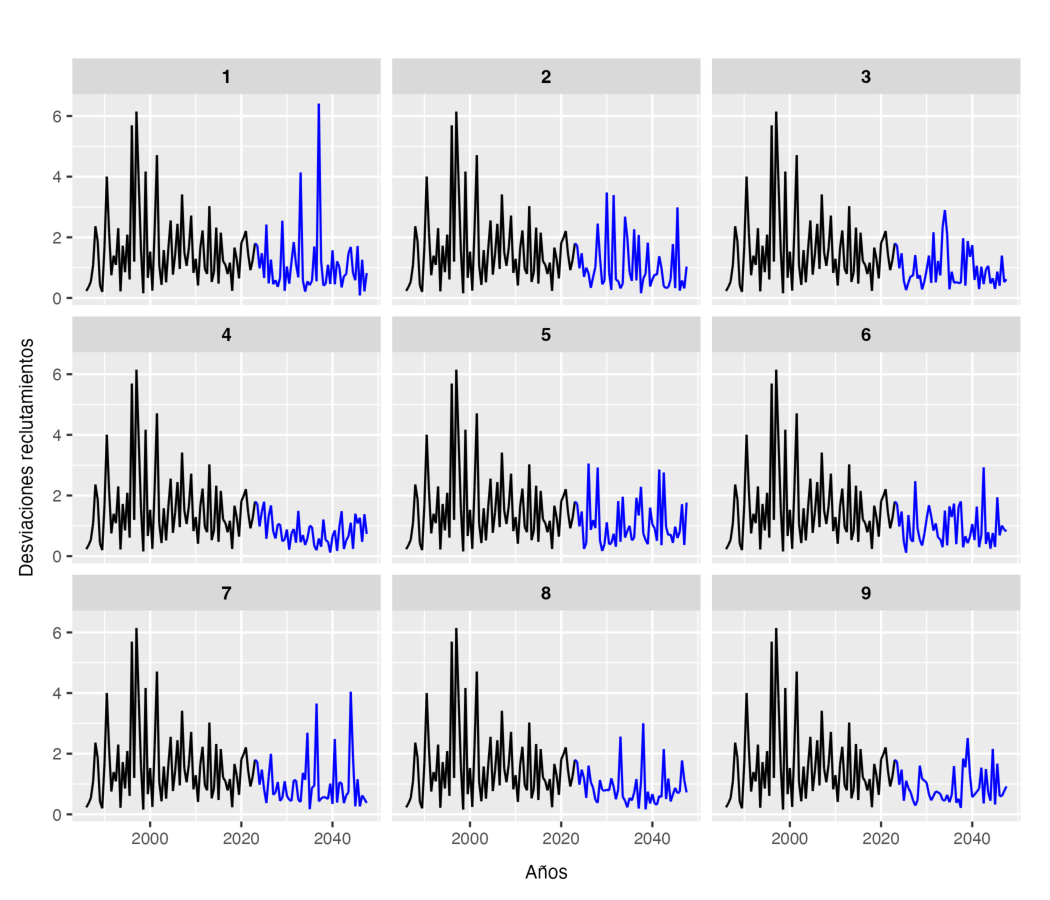
\includegraphics[scale=0.65]{figura5.pdf}
    \caption{. Desviaciones de los reclutamientos para seis simulaciones del stock de anchoveta para el modelo operativo caso base OM1. Las líneas negras indican las desviaciones de los reclutamientos durante el período histórico (igual para todas las simulaciones), y las líneas azules indican las desviaciones de los reclutamientos en el período de proyección, las cuales fueron generadas a partir de una distribución de probabilidad (desviación estándar y auto-correlacionada).}
    \label{fig:figura5}
\end{figure}

\subsection{Parámetros de historia de vida}

Respecto a este tema, la discusión estuvo asociada a los parámetros de crecimiento y la ojiva de madurez. Los parámetros de crecimiento supuestos para el acondicionamiento de los modelos operativos se basaron en la lectura de macro anillos (Plaza et al. 2012), y la lectura de micro anillos diarios (Cerna and Plaza, 2016). Una vez definidos los parámetros de crecimiento, se discutió sobre la ojiva de madurez presentada por Hernández et al. (2022). Estos resultados fueron expuestos durante el taller, donde se confirma una disminución de la talla media de madurez (L50), con una determinada variabilidad interanual (ver Figura 3 para el detalle de los escenarios alternativos). 

\subsection{Selectividad}

El patrón de selectividad para cada flota se mantuvo de acuerdo con la configuración y cambio temporal incluidos en el actual modelo de evaluación de stock para el stock de anchoveta. 

\subsection{Error de implementación}

No hay errores de implementación explícitos en el MO. Sin embargo, de la manera que está diseñado, este error se encuentra implícito en el PM. La “hiper-regla”, que opera en la pesquería de la anchoveta norte, determina que sin importar la CBA recomendada (en el hito 1 o 2), la CBA final siempre será la mayor de estas. De acuerdo con lo anterior, el error de implementación tiene lugar cuando la CBA adoptada es la recomendada en el primer hito.  

\subsection{Error de observación}

El error de la captura e índices de abundancia es tomado de los residuos del condicionamiento del MO. Los tamaños muestrales para la función de las muestras corresponden a los modelos de evaluación principalmente para la estructura de tamaño de la flota y crucero. Hay una diferencia entre la función de los tamaños muestrales y la función de probabilidad. El tamaño de muestra para la distribución multinomial de la composición para todas las flotas y el crucero fue fijado en 500 para representar un nivel de muestreo con alta precisión.
